\chapter{User interface} \label{cpt:gui}

\section{Purpose and functionality}
As the pure command line interface provided too few possibilities to see the
overall performance of our algorithms and lacks a simple way to execute
batches of runs, we decided to develop a small GUI in Swing to match these two
requirements.

The \texttt{SwingUI} only needs the \texttt{FileUtils} to run properly. As it
starts the \texttt{Runner} by simply calling its main method, there is no need
to make big adaptations to the \texttt{Runner} itself. Only, in order to prevent
the program from shutting down at any occuring error we had to replace the
\texttt{System.exit(0)} calls by simple \texttt{RuntimeException}s. And, in
order to make it run properly on Windows systems, we changed some code
regarding paths, that had hardcoded Unix path seperators (``/'').

Starting the program will allow you to select one or multiple files, which
should be located in the ``\texttt{./data/}'' folder. On the bottom of the
window three checkboxes let you choose, whether the output files should be
generated. The ``Run'' buttons on the top are pretty self-explanatory.

\section{Outputs}
The outputs are displayed seperately for Onsets, Tempo and Beat, to keep a
straight interface. Each of the three output tabs has the same layout:

\begin{itemize}
  \item In the upper half, each output file will be displayed. For onsets and
  beat, only the respective ``\texttt{*.eval}'' files appear, whereas for the
  tempo the ``\texttt{*.bpms}'' as well as the ``\texttt{*.bpms.eval}'' file.
  \item In the bottom half, the selected file will be displayed as well as the
  summary of this set of evaluations. To make differences easy to spot at first
  look, the summaries are color coded pretty straight forward: The greener, the
  better.
\end{itemize}

\begin{figure}[htp]
\begin{center}
  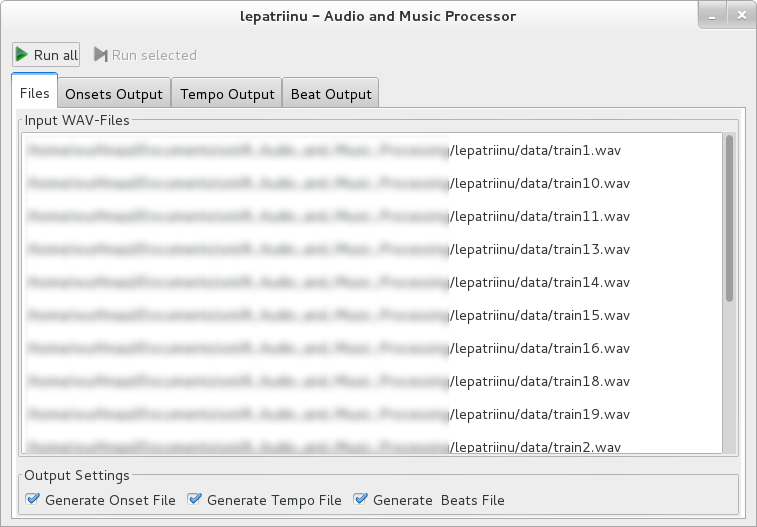
\includegraphics[width=\textwidth]{chapter/gui}
  \caption{Graphical user interface}
  \label{fig:gui}
\end{center}
\end{figure}

\begin{figure}[htp]
  \centering
  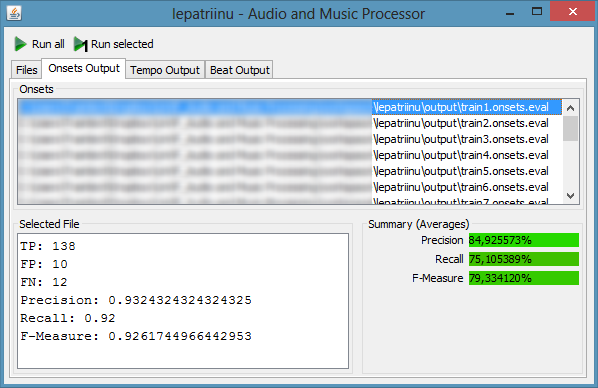
\includegraphics[width=\textwidth]{chapter/GUIOutput}
  \caption{The output of the onsets}
  \label{fig:guioutput}
\end{figure}